\chapter{Introduction to brain physiology and research methods}
\label{chap:introduction}

\section{Basic facts about the human brain}
The human brain is partitioned in many structures. The first one is the \textbf{cortex}, and in the following we provide the \textit{traditional function specializations} \notet:
\begin{itemize}
    \item \textbf{Temporal} lobe: \textbf{Auditory processing} (hearing and language);
    \item \textbf{Parietal} lobe: \textbf{Attention}, touch, saccade planning;
    \item \textbf{Frontal} lobe: Planning, execution, \textbf{higher level cognition}, high level language processing and language production;
    \item \textbf{Occipital} lobe: \textbf{Vision}, perception of visual features, categories and location.
\end{itemize}

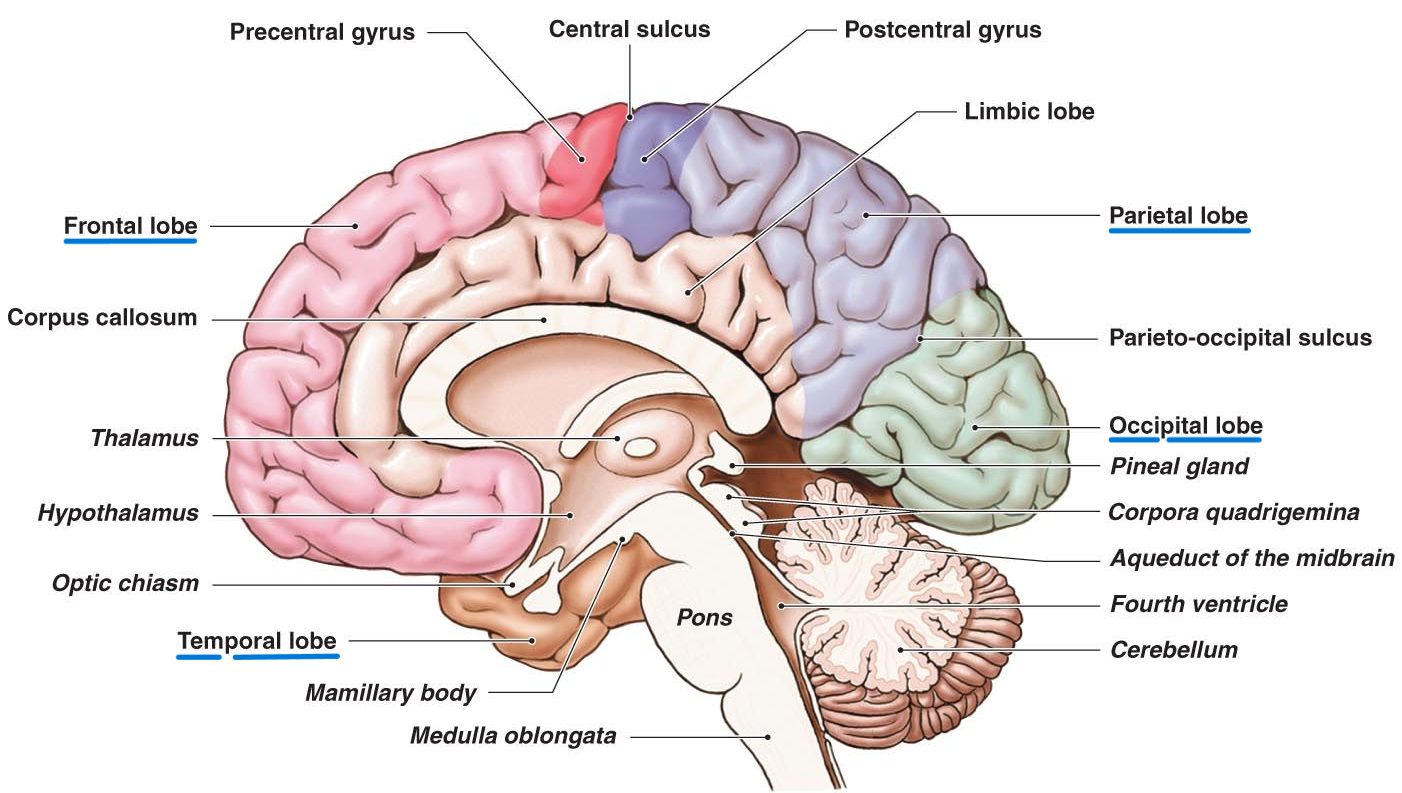
\includegraphics[width=\textwidth]{images/brain.png}

\osst{Here we have the traditional function specializations, even though nowadays we know that all areas of the brain take part in more functions: a function is computed by the whole network. The auditory processing is a sort of exception: audio is processed only in the temporal lobe; however, it is still part of the network, as its functions can be \textit{modified on demand}.}

We then have the \textbf{subcortical structures}:
\begin{itemize}
    \item \textbf{Cerebellum}: fine motor control, implicated in emotional responses;
    \item \textbf{Thalamus}: Major gateway for sensory processing. One of the final stops before sensory information arrives at the cortex;
    \item \textbf{Hippocampus}: implicated in construction of memories; these are later transferred to other cortical regions;
    \item \textbf{Corpus Callosum}: a main ``highway" of white matter tracks that connects the two hemispheres.
\end{itemize}

\subsection{Gray matter}
Gray matter (GM), which gets its name from its color, is the brain part that \textbf{performs computation}. The gray matter includes not only the cerebral cortex but also the cerebellum, basal ganglia, thalamus, and several other regions. Techniques for measuring brain activity often reflect the function of gray matter regions, which are responsible for the majority of cognitive processing. As a result, understanding the role and function of gray matter in the brain is essential for gaining insight into various neurological and psychiatric conditions.

\begin{wrapfigure}[10]{r}{0pt}
  \centering
  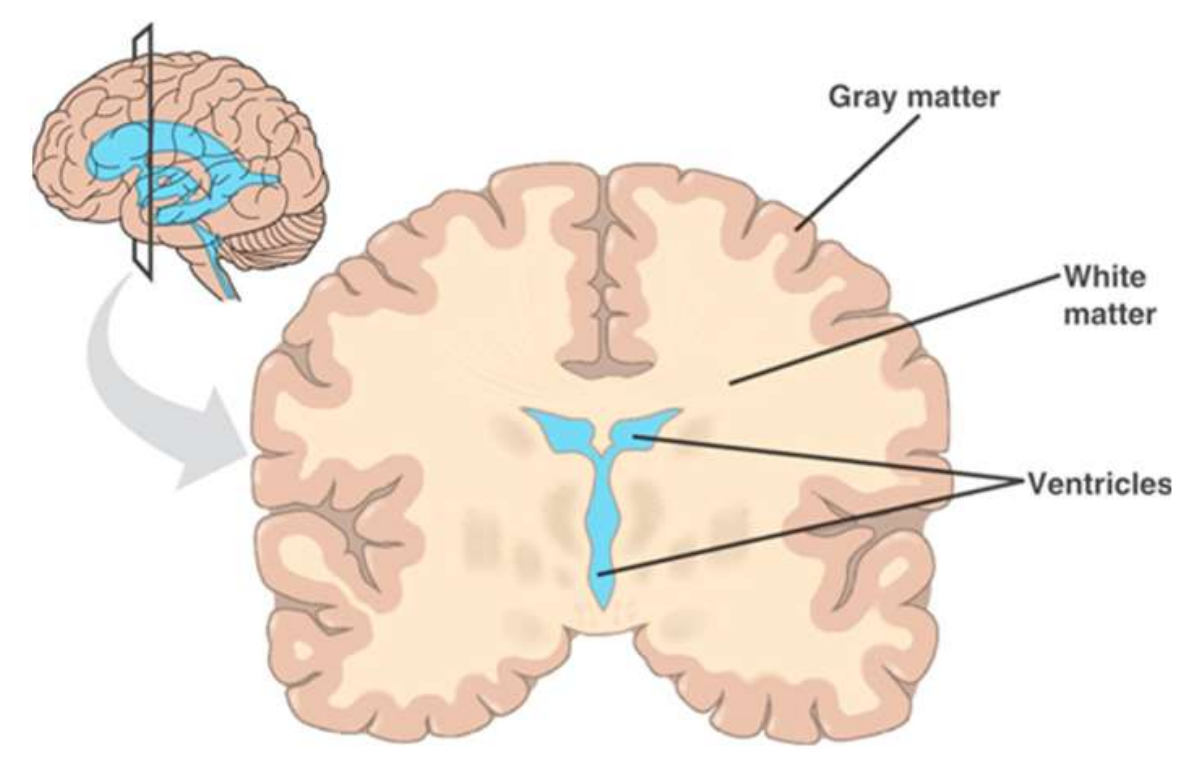
\includegraphics[width=0.4\textwidth]{images/brain_2.png}
\end{wrapfigure}

The gray matter is on the perimeter of the brain, and its folded structure (with \textit{gyri} and \textit{sulci}, determined by the DNA) allows for higher surface. This also causes parts that are located close to each other, in physical space, to be far away in cortical space.

\subsection{White matter}
White matter consists mainly of \textbf{long-range axon pathways}, or \textit{tracts}, that \textbf{connect different regions of the brain}. Unlike gray matter, there is \textbf{no direct information processing} within white matter itself. The structure of white matter can change with learning because it reflects the long-range neural pathways that carry nerve impulses and facilitate the communication between different regions of the brain. 

% \begin{wrapfigure}{l}{0.4\textwidth}
\begin{wrapfigure}[15]{l}{0pt}
  \centering
  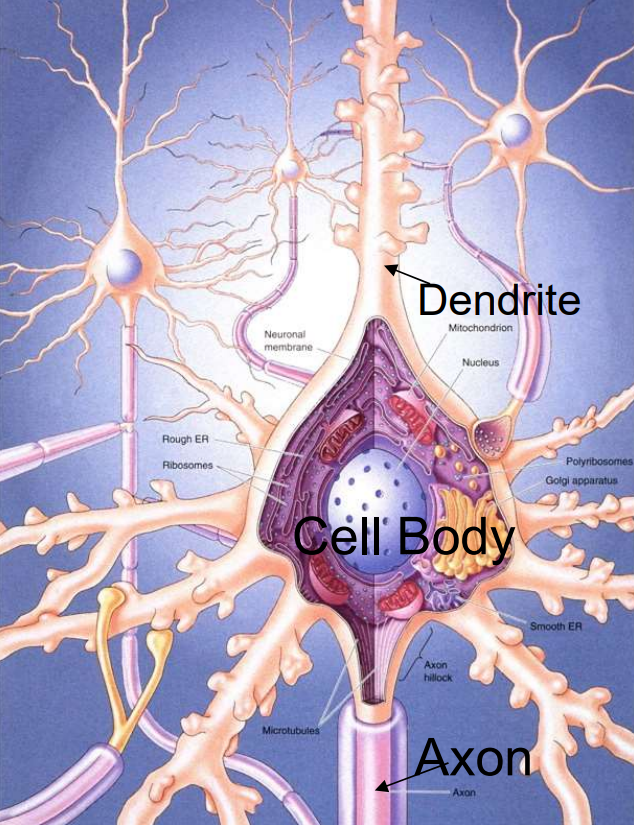
\includegraphics[width=0.3\textwidth]{images/neuron.png}
\end{wrapfigure}
Damage to white matter, such as the loss of myelin in conditions like multiple sclerosis, can have significant impacts on communication between different regions of the brain, leading to various neurological and psychiatric symptoms. Therefore, understanding the role and function of white matter is critical for studying brain function and identifying potential targets for interventions in various neurological and psychiatric disorders.

\subsection{The neuron}
A neuron consists of \textbf{dendrites}, a \textbf{cell body} (aka \textbf{soma}) and an \textbf{axon}. Connections between neurons are called \textbf{synapses}, and typically occur on a neuron's dendrite (but in some cases also on soma), which receives synaptic signals. Synapses are \textbf{chemical}, \textbf{not electrical}.
A neuron will \textit{fire} (generate an action potential) depending on the number of signals it receives on its dendrites and their strength, which are \textit{summed} in the neuron's body. 

\details{Digression: Synaptic communication}{Synaptic communication is the process by which neurons communicate with each other through the release and reception of chemical signals called neurotransmitters. The postsynaptic neuron receives the signal, which is either excitatory (the neuron is depolarized and fires an action potential), or inhibitory (causing the neuron to hyperpolarize and become less likely to fire an action potential). Depolarization produces an \textit{all-or-nothing} signal: \textbf{no partial firing}.
}

\subsection{Neuroplasticity}
Neuroplasticity refers to \textit{network changes} over time, to adapt to the environment.
Synapses can be \textit{strengthened} or \textit{pruned}.

\begin{wrapfigure}[12]{r}{0pt}
  \centering
  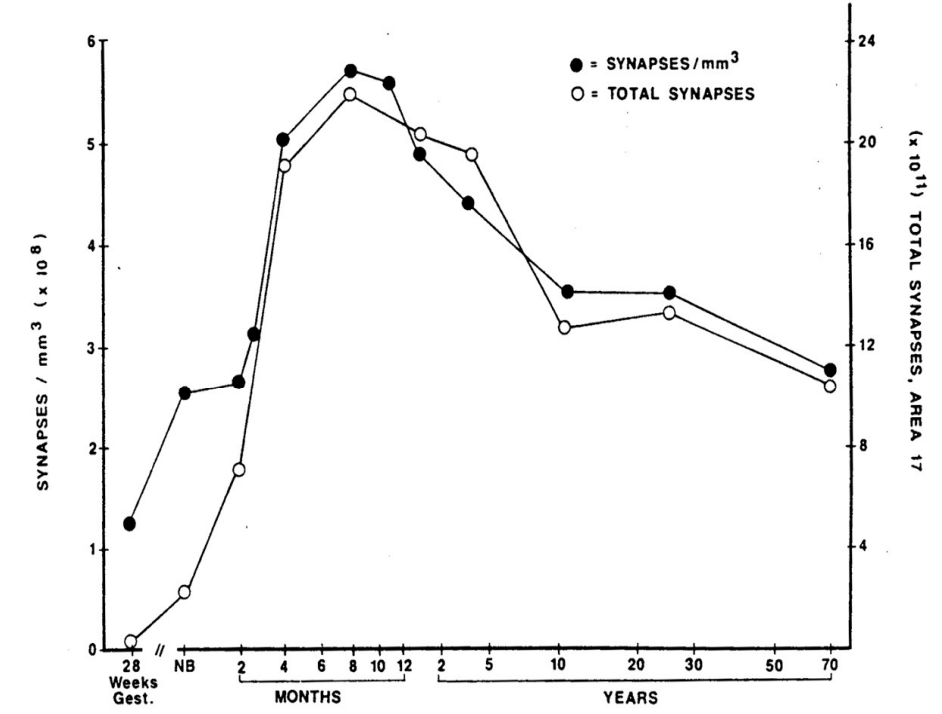
\includegraphics[width=0.35\textwidth]{images/neuroplasticity.png}
  \caption*{Synaptic density and total synapses in visual cortex as a function of age.}
\end{wrapfigure}
Connections between neurons are consistently removed (or created) depending on use.
A large percentage of neurons that develop die. A \textit{hub} neuron, which receives inputs from many neurons is more likely to survive. When many neurons connect to a target neuron, this decreases their survival rate. This calibration is thought to be associated with generating an optimal degree of 
synaptic connection.
Brain volume triples between birth and adulthood; this is mostly not due to addition of neurons, but to an increased number of connections (synapses), myelination of existing axons and greater dendritic branching.

\section{Studying the human brain: tools and basics of experimentation}
The human brain can be studied at different levels of organization, from systems and pathways to synapses and membranes.
\begin{itemize}
    \item Systems and pathways: large-scale neural networks responsible for specific functions, such as sensory perception, motor control, and cognition. These may be topographically distributed.
    \item Circuits and neurons: networks of interconnected neurons that underlie information processing within the brain.
    \item Synapses and membranes: molecular and cellular mechanisms that govern the transmission of signals between neurons, such as the release of neurotransmitters and activation of ion channels.
\end{itemize}
Studying the brain at different scales provides insights into organization of function from the macroscopic to the microscopic level.

\subsection{Basics of experimentation}
There are several \textbf{non-invasive tools} available for studying brain activity and structure, including electroencephalography (EEG), structural imaging, functional magnetic resonance imaging (fMRI), and diffusion-weighted imaging. These tools provide insights into different aspects of brain function and structure: electrical activity of neurons, structural connectivity of brain regions, and metabolic activity (i.e., energy consumption) associated with specific tasks or behaviors.

\begin{figure}[ht]
    \centering
  \captionsetup{width=.8\linewidth}
    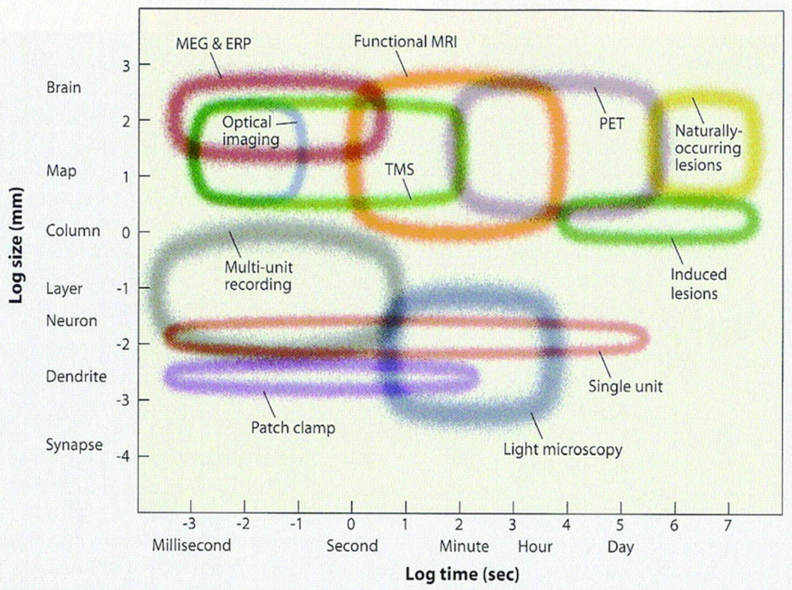
\includegraphics[width=0.7\textwidth]{images/tools.png}
    \caption{\textbf{Temporal} and \textbf{spatial resolution} of common tools. An additional dimension is \textbf{coverage}: how much of the brain is simultaneously observable by the tool.}
\end{figure}
Experimental procedures are used to analyze the data collected by these tools; they typically consist in conducting studies that involve manipulating variables of interest and collecting and analyzing data from participants. In neuroscience, an \textbf{experiment} or study is a systematic \textbf{investigation of a research hypothesis} that involves \textbf{manipulating variables and measuring their effects on some outcome of interest}.
Conclusions from experiments are drawn by analyzing the data collected from participants and testing whether there are statistically significant differences between groups or conditions, typically using statistical methods to quantify the strength and direction of effects and assessing the probability that the observed effects are due to chance.\\

In the following sections we will discuss the most important tools (namely EEG, structural imaging, fMRI), however there are many others:
\begin{itemize}
    \item TMS (Transcranial Magnetic Stimulation): induces a virtual lesion of a part of the brain (this might be dangerous).
    \item MEG (Magnetoencephalography): directly measures the magnetic fields generated by neural activity.
    \item Patch clamp: records the current from ion channels in the cell membrane.
\end{itemize}

\subsection{Electroencephalography (EEG)}
EEG is a non-invasive method used to study patterns of brain activity with high temporal resolution.
The principle behind EEG is that it is sensitive to very subtle changes in electric potentials below the sensors, which are propagated to the scalp. These changes reflect alterations in the electrical environment of thousands of neurons that fire in synchrony. Each EEG sensor gives one time series.
It is difficult to pinpoint the brain regions causing the fluctuations, since the electromagnetic waves are dispersed by the scalp. However, the \textbf{timing of the signals is very precise}.

\subsubsection{From EEG time series to ERP}
\begin{wrapfigure}[13]{r}{0pt}
  \centering 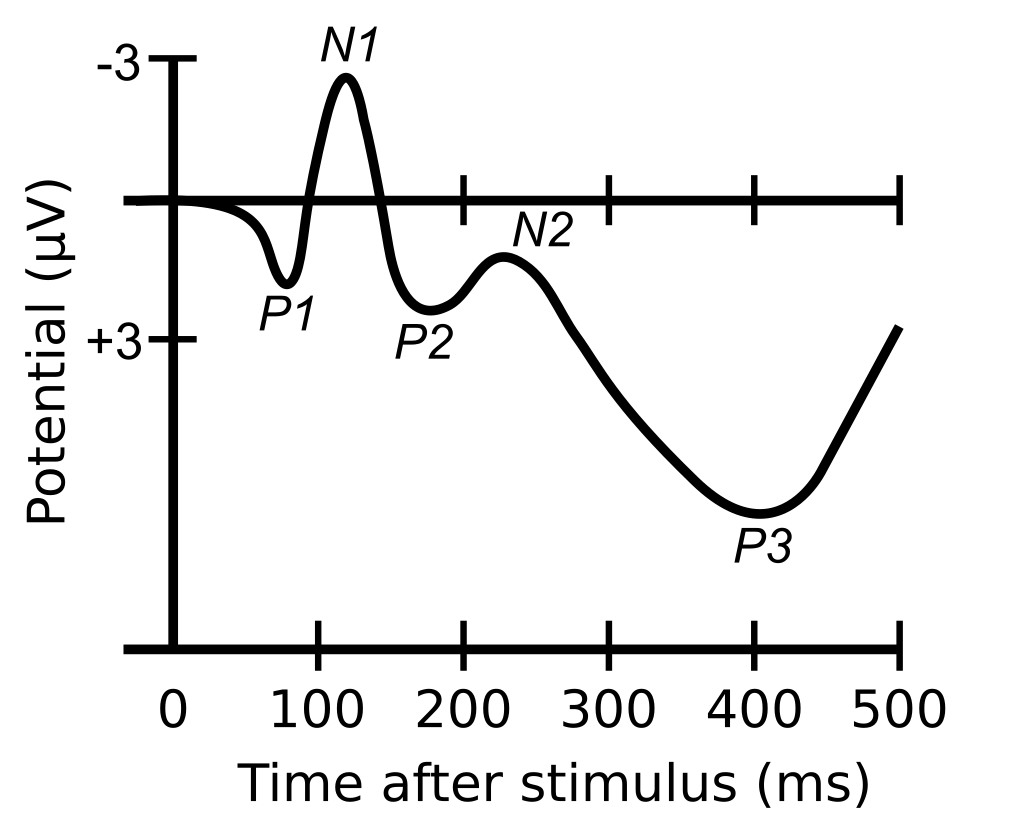
\includegraphics[width=0.3\textwidth]{images/ComponentsofERP.png}
  \caption*{A waveform showing several ERP components. Notice the plot has negative voltages upward.}
\end{wrapfigure}

Tasks can generate \textbf{stereotyped evoked potentials} that can be averaged (over all epochs \notet) to obtain an \textbf{Event-Related Potential} (aka \textbf{Evoked-Response-Potential}). An ERP analysis quantifies electrical brain responses to events/stimuli based on time-locked EEG portions. This analysis can be used as the basis for more sophisticated analysis such as source localization.

\osst{An epoch consists in the timespan [0ms, 500ms] after the stimulus presentation.}

Neural activity is not the only activity causing electrical fluctuations. Muscles are also one of the main causes of fluctuations (e.g., every time we blink or move our eyes there are oscillations collected by EEG sensors). All these \textbf{noise} artifacts have to be independently measured and then removed from the data. The sensors placed near the eyes are indeed used to measure such noise.
Moreover, since the interesting brain \textbf{signal is low}, while the \textbf{noise is high}, \textbf{many repetitions} of each condition are needed (the impact of noise on computing ERPs scales down as a function of the square root of the number of observations). This noise reduction applies to each timepoint measured. 
The need for many repetitions can be challenging and time-consuming, but it is necessary for obtaining reliable and statistically significant results. In addition to repetition, other techniques such as filtering and artifact rejection can also help to reduce noise in EEG recordings.\\

EEG also contains important information in form of frequency characteristics (cycling rate). The frequency differentiates sleep stages from awake, and drowsy from alert.
Power plots can show the relative strength of each frequency, helping in \textit{frequency band interpretation}. For instance, the alpha band in EEG, which has a frequency range of 8-12 Hz, is commonly observed during eyes-closed recordings and relaxed states. Alpha oscillations are associated with reduced communication between the cortex and thalamus. During externally oriented attention and stimulus processing, the alpha activity is suppressed.

\boxc{ERP in practice}{
This experiment tries to understand when children develop the ability to predict language. It consists in presenting congruous (e.g., \textit{pizza was too hot to eat}, in blue) or incongruous (e.g., \textit{pizza was too hot to \textbf{sit}}, in red) sentences.

\begin{center}
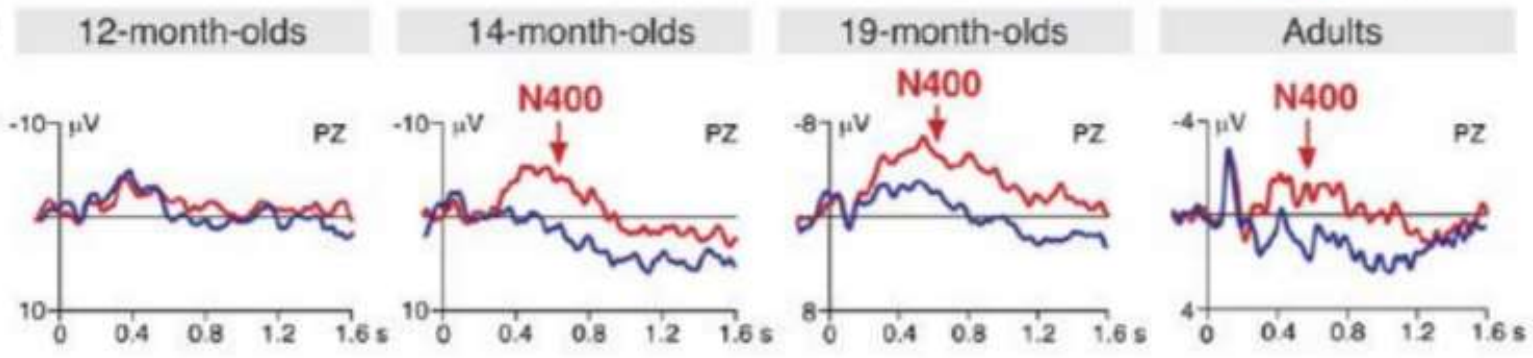
\includegraphics[width=0.8\textwidth]{images/ERP.png}
\end{center}

Here we see the ERPs from a single sensor (the PZ one). We can notice the time point where the two functions diverge is when the word is processed by the brain (so we can understand how much it takes for a word to be processed).
}

\subsection{Structural imaging}
Structural imaging involves collecting 3D images of the brain, similar to the images obtained in a medical setting.

\begin{center}
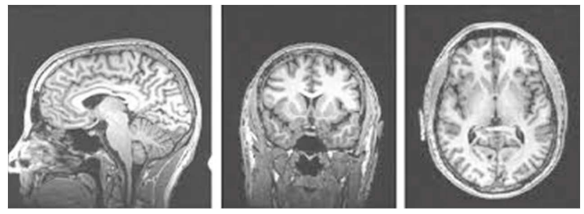
\includegraphics[width=0.7\textwidth]{images/structural_imaging.png}
\end{center}

\begin{wrapfigure}[6]{r}{0pt}
  \centering 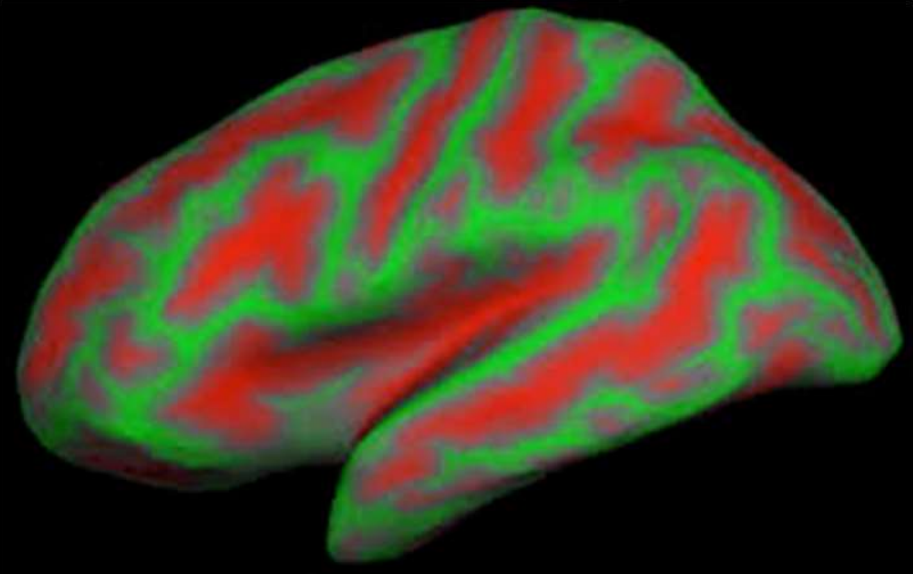
\includegraphics[width=0.3\textwidth]{images/thickness.png}
  \caption*{Example of cortical thickness map.}
\end{wrapfigure}
This type of imaging can provide information about various aspects of brain 
structure, such as:

\begin{itemize}
    \item Gray matter volume (i.e., the overall size of the gray matter in the brain);
    \item The density of gray matter in specific regions, which can approximate the concentration of neurons;
    \item Cortical thickness at a resolution of a few millimeters;
    \item Surface area of particular brain regions.
\end{itemize}

Calculation of cortical thickness is usually done by converting the brain's 3D representation to a 2D sheet representation.
We can look for correlation (covariance across different people) of structural cortical thickness between different areas of the brain.

\subsection{Functional  magnetic resonance imaging (fMRI)}
Functional MRI is the method that helped most in understanding how the brain works. It consists in observing which parts of the brain are involved in \textbf{metabolic activity} when we do things like thinking or perceiving \notet.

FMRI uses a big magnet to affect protons in the brain and then measures how they behave as they return to their original state (areas that are involved in oxygen consumption have a different relaxation profile).
By analyzing the patterns of proton behavior, we can identify which brain areas are more active during certain tasks.
This method gives us very detailed information about where activity is happening in the brain and can help us understand how different regions contribute to complex processes like thinking and perception.
With fMRI we get a time series for each \textbf{voxel} (typically a $3\times3\times3$ mm brain region).

\osst{In neurology, metabolic activity is often used as a proxy for neural activity: active neurons require more energy to function and can increase their metabolic rate.}

In our brain there are 60 to 70 thousands voxels. By chance (statistics) we will surely get some false positives. For this reason we undertake many experiments.

\boxc{fMRI in an experimental context}{
The \textbf{signal} is defined as the measurable response to a stimulus.\\
In statistical detection theory we:
\begin{itemize}
    \item understand relationship between stimulus and signal;
    \item describe noise properties statistically;
    \item devise methods to distinguish noise-only measurements from signal+noise measurements, and assess the methods' reliability.
\end{itemize}

\textit{Stimulus-signal connection} and \textit{noise statistics} are complex and poorly characterized.
We devise, a priori, a \textbf{mathematical model connecting stimulus} (or ``activation”) \textbf{to signal} (typically a regression model).
We make an estimation of the \textbf{statistical model for the noise}, taking into account whether it is random, structured, oscillatory, etc.
These two models are then combined to produce an \textbf{equation for measurements given signal+noise} (also often a regression model).
The final result is an equation with few \textbf{free parameters that can be fitted to the data}.\\

FMRI analysis often fits a (convolved) activation model to \textbf{each voxel's time series separately} (\textit{massively univariate analysis}).
Pre-processing techniques are applied to reduce noise, including spatial smoothing across nearby voxels.
The outcome of model fitting is a collection of parameters estimated from each voxel's data. The Activation Amplitude (Beta) is the most critical parameter, and it is related to the correlation between the model and activity.
At the group level, the \textbf{voxel-level estimates are pooled together to reach a group-level conclusion per voxel}.\\

FMRI measures changes in neural activity, there are no absolute magnitudes.
The baseline signal level in a voxel does not provide information about neural activity.
An experiment using fMRI requires at least two conditions to detect changes in neural activity. Minimally, experiments use a ``task" and ``rest" condition. In such a two-task experiment intermixed with rest, a Beta value is estimated per task, and their values are contrasted to determine the difference between the two tasks.
}
\begin{wrapfigure}[8]{r}{0pt}
  \centering
  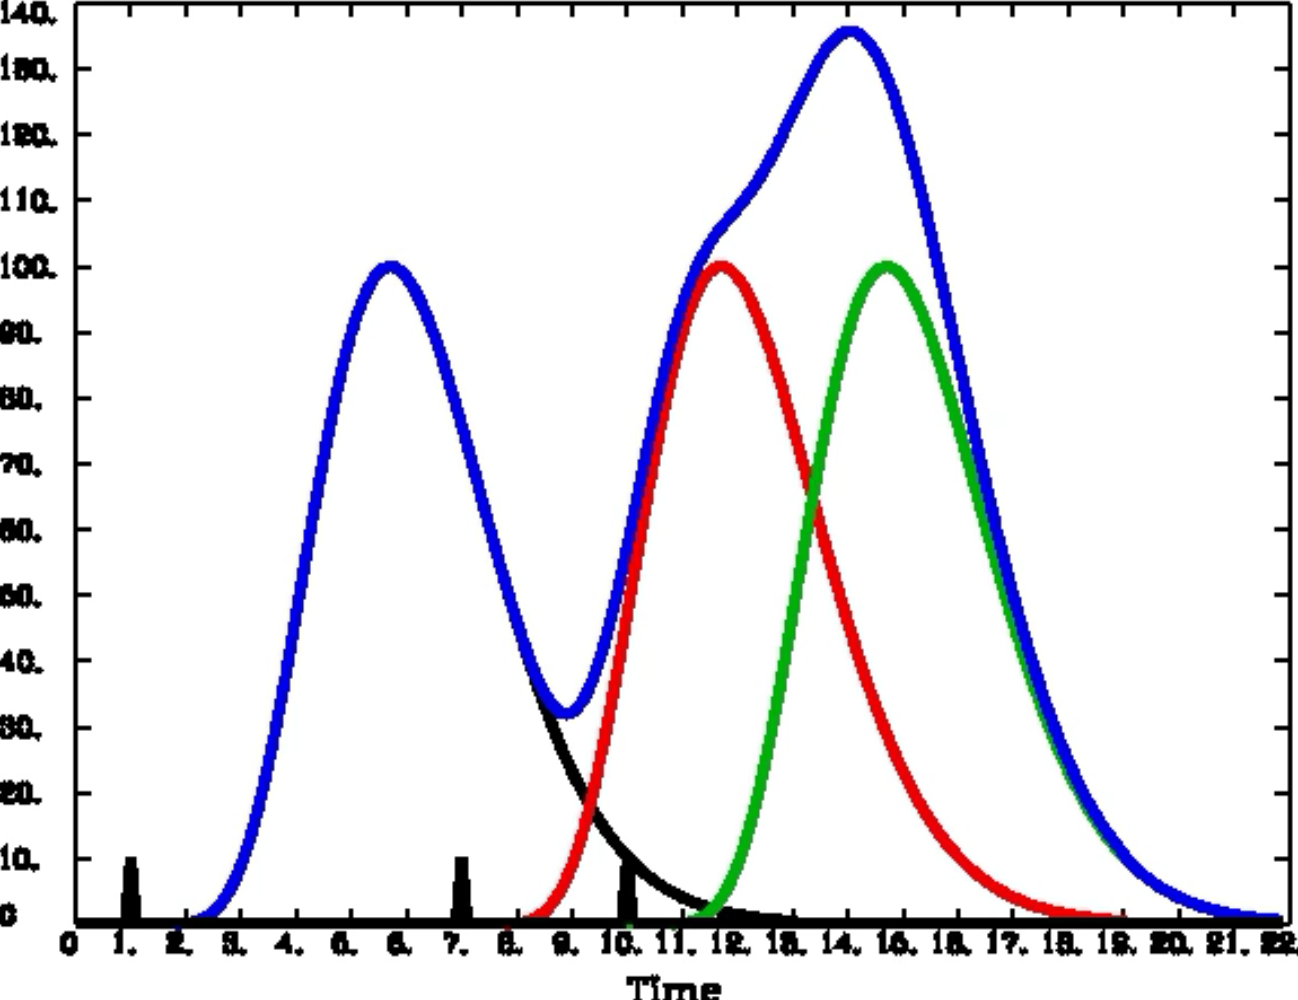
\includegraphics[width=0.3\textwidth]{images/hrf.png}
\end{wrapfigure}

\subsubsection{Hemodynamic response function (HRF)}
The response measured by fMRI (called ``Hemodynamic" because it is related to blood) is delayed since the blood requires time to flow. Notice this is not a simply shifted impulse response, as it is a smooth function.
For this reason, fMRI tells us \textbf{where} the process takes place, but not \textbf{when}. Combining fMRI and EEG can be a solution.

\subsection{Diffusion weighted imaging (DTI)}
Diffusion weighted imaging (also known as \textbf{Diffusion MRI} or \textbf{Diffusion tensor imaging}), is used to examine the structure of \textbf{white matter fibers}.
For each voxel, the preferred \textbf{direction} of diffusion and the \textbf{strength} of diffusion are estimated to determine white matter tracts.
These connections are considered \textit{hardwired} connections. They can be cross-referenced against functional connectivity.
